
\titleformat{\chapter}{\bfseries \large \center}{PHỤ LỤC \thechapter.}{0.3em}{}[]

%\addcontentsline{toc}{chapter}{{\bf PHỤ LỤC}}
\thispagestyle{empty}

\appendix

\chapter[MỘT SỐ CÔNG THỨC TOÁN HỌC THƯỜNG GẶP]{MỘT SỐ CÔNG THỨC \\TOÁN HỌC THƯỜNG GẶP} \label{plvanbanphapquy}


\[
\tilde f(\omega)=\frac{1}{2\pi}
\int_{-\infty}^\infty f(x)e^{-i\omega x}\,dx\,,
\]
\[
\dot{\vec \omega}=\vec r\times\vec I\,
\]
\[
\exp(i\theta)=\cos\theta +i\sin\theta\,,\quad
\sinh(\log x)=\frac{1}{2}\left( x-\frac{1}{x} \right).
\]
Một số hàm có dạng phức tạp:
\[
\lim_{q\to\infty}\|f(x)\|_q 
=\max_{x}|f(x)|,
\]
\begin{eqnarray*}
	e^x & = & \sum_{n=0}^\infty \frac{x^n}{n!}
	\quad\text{với }n!=\prod_{i=1}^n i\,,  \\
	\overline{U_\alpha} & = & \bigcap_\alpha U_\alpha\,.
\end{eqnarray*}

Biểu thức có dạng rút gọn: \(
1/(1-x)=\sum_{n=0}^\infty x^n
\) trong một dòng mà vẫn bảo đảm độ giãn dòng không thay đổi.

\[
\begin{matrix}
	-2 & 1 & 0 & 0 & \cdots & 0  \\
	1 & -2 & 1 & 0 & \cdots & 0  \\
	0 & 1 & -2 & 1 & \cdots & 0  \\
	0 & 0 & 1 & -2 & \ddots & \vdots \\
	\vdots & \vdots & \vdots & \ddots & \ddots & 1  \\
	0 & 0 & 0 & \cdots & 1 & -2
\end{matrix}
\]

\[ f(n) = \left\{ 
\begin{array}{l l}
n/2 & \quad \text{nếu $n$ chẵn}\\
-(n+1)/2 & \quad \text{nếu $n$ lẻ}
\end{array} \right.\]

\[
A_{m,n} =
\begin{pmatrix}
	a_{1,1} & a_{1,2} & \cdots & a_{1,n} \\
	a_{2,1} & a_{2,2} & \cdots & a_{2,n} \\
	\vdots  & \vdots  & \ddots & \vdots  \\
	a_{m,1} & a_{m,2} & \cdots & a_{m,n}
\end{pmatrix}
\]

\begin{equation}
x = a_0 + \cfrac{1}{a_1
	+ \cfrac{1}{a_2
		+ \cfrac{1}{a_3 + \cfrac{1}{a_4} } } }
\end{equation}

\newpage
\chapter[MỘT SỐ VÍ DỤ VỀ LỆNH VẼ  \LaTeX CỦA GÓI TIKZ]{MỘT SỐ VÍ DỤ VỀ LỆNH VẼ \LaTeX \\ CỦA GÓI TIKZ}

%Các ví dụ dưới đây không phải là ảnh bitmap mà là hình vector được vẽ bằng các câu lệnh \LaTeX  %trong gói \textbf{tikz}.

\section{Ví dụ 1 - câu lệnh biểu diễn công thức hóa học}
\ttfamily
\footnotesize

%\pagestyle{empty}

\begin{center}
	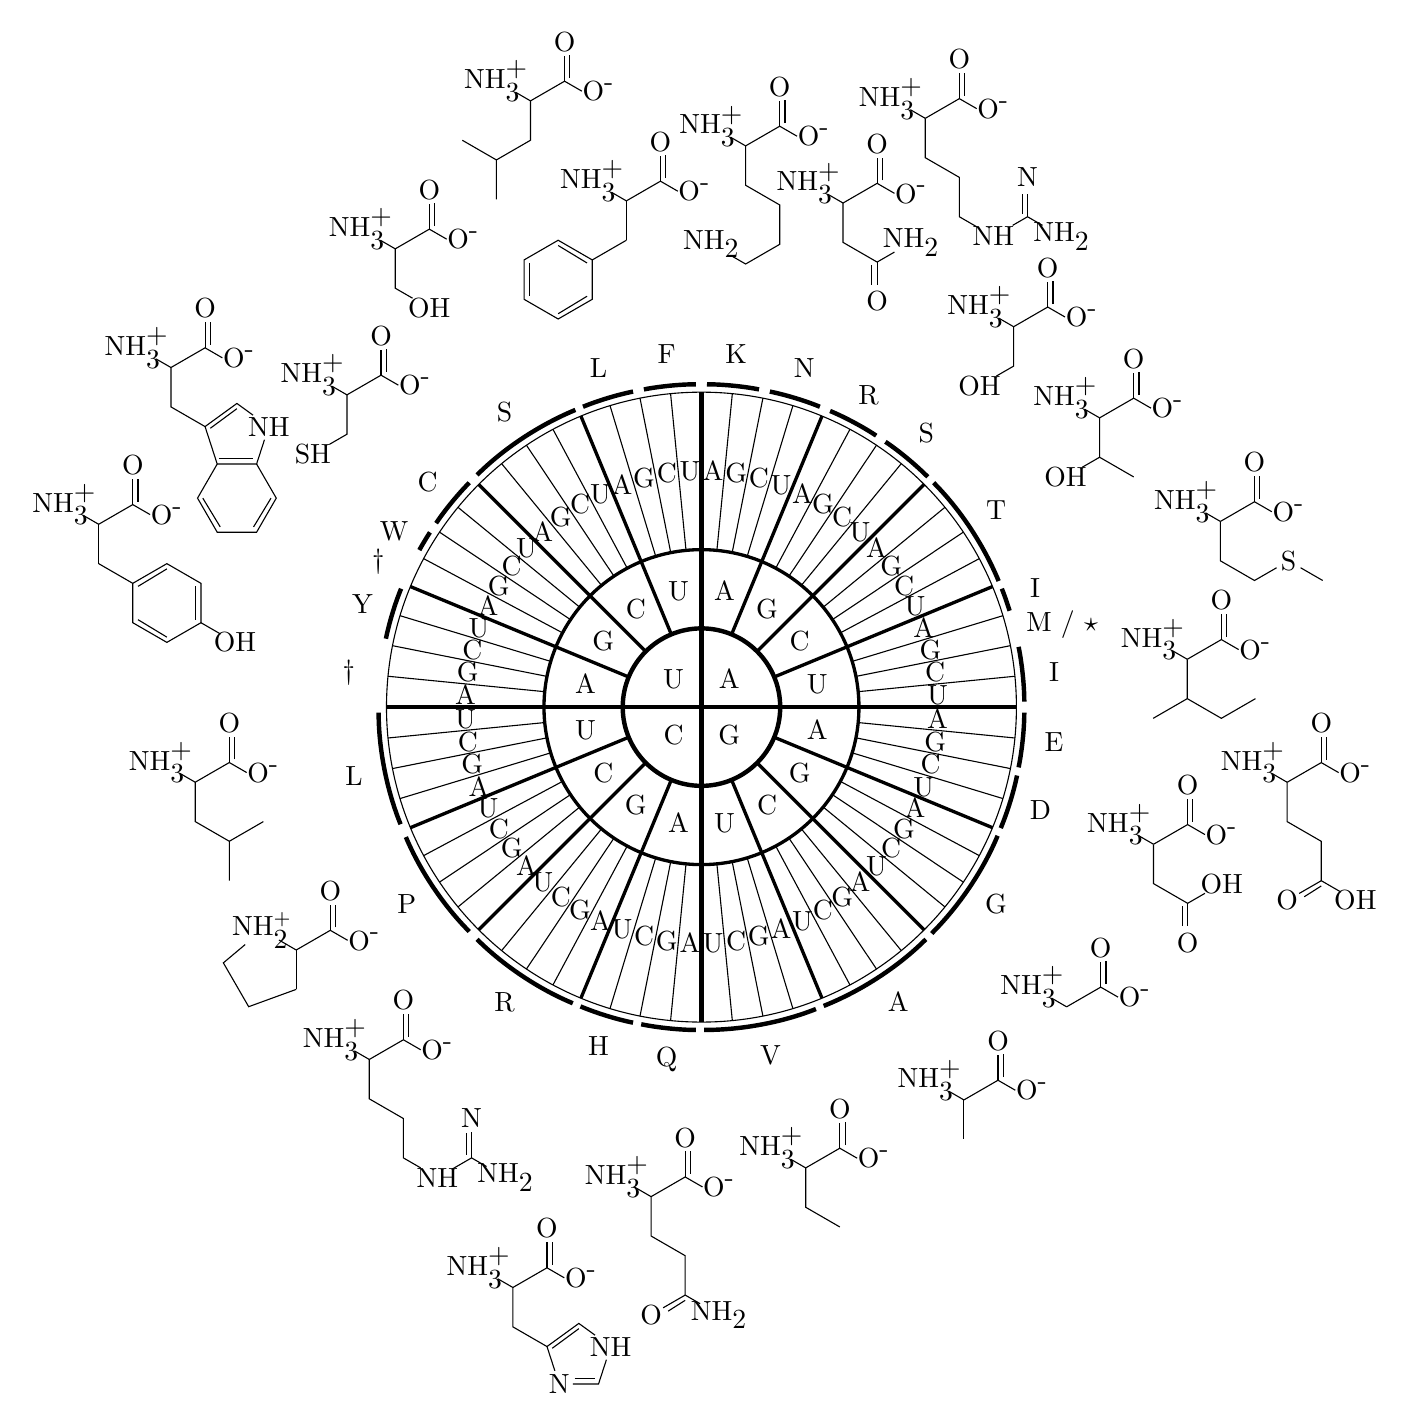
\begin{tikzpicture}
	\tikzstyle{every node}=[inner sep=1.7pt,anchor=center]
	%	to_x and from_x styles denote bonds terminating or starting in labeled nodes. x denotes the number of letters in the node label.
	\tikzstyle{to_1}=[shorten >=5pt]
	\tikzstyle{to_1i}=[shorten >=6pt]
	\tikzstyle{to_2}=[shorten >=7pt]
	\tikzstyle{to_3}=[shorten >=8pt]
	\tikzstyle{from_1}=[shorten <=5pt]
	\tikzstyle{from_1i}=[shorten <=6pt]
	\tikzstyle{from_2}=[shorten <=8pt]
	\begin{scope}
	\draw [ultra thick] circle(1cm);
	\draw [ultra thick] (0:4)--(180:4) (90:4)--(270:4);
	\foreach \a/\l in {45/A,135/G,225/C,315/U}{
		\node at (90-\a:0.5cm) {\l};
	}
	\draw [very thick] circle(2cm);
	\foreach \A in {90,0,270,180}{
		\foreach \a/\l in {22.5/A,45/G,67.5/C,90/U}{
			\draw [very thick] (\A+\a:1) -- (\A+\a:4);
			\node at (\A-\a+11.25:1.5) {\l};
		}
	}
	\draw circle(4cm) (0:4)--(180:4) (90:4)--(270:4);
	\foreach \A in {90,180,270,0}{
		\foreach \a in {0,22.5,45,67.5}{
			\foreach \i/\l in {5.625/A,11.25/G,16.875/C,22.5/U}{
				\draw (\A+\a+\i:2) -- (\A+\a+\i:4);
				\node at (\A-\a-\i+2.8125:3) {\l};
			}
		}
	}
	\end{scope}
	\begin{scope}[scale=0.5]	% Lysine
	\draw[ultra thick,shorten >=2pt,shorten <=2pt] (90:8.2)
	arc(90:90-2*5.625:8.2);
	\path (90-0.8*5.625:14.3) node (zero) {};
	\draw[to_2]  (zero.center)	-- ++(30:1) node (CO) {}  
	-- +(330:1) node [anchor=base] {O$^{\mbox{-}}$};
	\draw[to_1]  (CO.center) 	-- +(90:1) node (Od) {O};
	\draw[to_1i] (CO.30)		-- +(90:1);
	\draw[to_3]  (zero.center)	-- ++(150:1) node {NH$_{\mbox{3}}^{\mbox{+}}$};
	\draw[to_3]  (zero.center)	-- ++(270:1) node(Cb){}
	-- ++(330:1) node (Cc) {}
	-- ++(270:1) node (Cd) {}
	-- ++(210:1) node (Ce) {}
	-- ++(150:1) node (Cf) {NH$_{\mbox{2}}$};
	\end{scope}
	\begin{scope}[scale=0.5]	% Asparagine
	\draw[ultra thick,shorten >=2pt,shorten <=2pt] (90-2*5.625:8.2)
	arc(90-2*5.625:90-4*5.625:8.2);
	\path (90-3.5*3.625-3:13.3) node (zero) {};
	\draw[to_2]  (zero.center)	-- ++(30:1) node (CO) {} 
	-- +(330:1) node [anchor=base] {O$^{\mbox{-}}$};
	\draw[to_1]  (CO.center)	-- +(90:1) node (Od) {O};
	\draw[to_1i] (CO.30)		-- +(90:1);
	\draw[to_3]  (zero.center)	-- ++(150:1) node {NH$_{\mbox{3}}^{\mbox{+}}$};
	\draw[to_2]  (zero.center)	-- ++(270:1) node(Cb){}
	-- ++(330:1) node (Cc) {}
	-- +(30:1) node (Cd) {NH$_{\mbox{2}}$};
	\draw[to_1i] (Cc.center)	-- +(270:1) node (O) {};
	\draw[to_1]  (Cc.210)		-- (O.150);
	\path (O.center) node {O};
	\end{scope}
	\begin{scope}[scale=0.5]	% Arginine
	\draw[ultra thick,shorten >=2pt,shorten <=2pt] (90-22.5:8.2)
	arc(90-22.5:90-33.75:8.2);
	\path (90-3.7*5.625:16) node (zero) {};
	\draw[to_2]  (zero.center)	-- ++(30:1) node (CO) {}
	-- +(330:1) node [anchor=base] {O$^{\mbox{-}}$};
	\draw[to_1]  (CO.center)	-- +(90:1) node (Od) {O};
	\draw[to_1i] (CO.30)		-- +(90:1);
	\draw[to_3]  (zero.center)	-- ++(150:1) node {NH$_{\mbox{3}}^{\mbox{+}}$};
	\draw[to_2]  (zero.center)	-- ++(270:1) node(Cb){}
	-- ++(330:1) node (Cc) {}
	-- ++(270:1) node (Cd) {}
	-- ++(330:1) node (NH1) {NH};
	\draw[from_2,to_3]  (NH1.center)	-- ++(30:1) node (Ce) {}
	-- ++(330:1) node {NH$_{\mbox{2}}$};
	\draw[to_1i] (Ce.center)	-- ++(90:1) node (N2) {};
	\draw[to_1]  (Ce.150)		-- (N2.210);
	\path (N2) node {N};
	\end{scope}
	\begin{scope}[scale=0.5]	% Serine
	\draw[ultra thick,shorten >=1pt,shorten <=2pt] (90-22.5-2*5.625:8.2)
	arc(90-33.75:90-33.75-11.25:8.2);
	\path (90-7*5.625:12.5) node (zero) {};
	\draw[to_2]  (zero.center)	-- ++(30:1) node (CO) {}
	-- +(330:1) node [anchor=base] {O$^{\mbox{-}}$};
	\draw[to_1]  (CO.center)	-- +(90:1) node (Od) {O};
	\draw[to_1i] (CO.30)		-- +(90:1);
	\draw[to_3]  (zero.center)	-- ++(150:1) node {NH$_{\mbox{3}}^{\mbox{+}}$};
	\draw[to_2]  (zero.center)	-- ++(270:1) node(Cb){} -- ++(210:1) node (Cc) {OH};
	\end{scope}
	\begin{scope}[scale=0.5]	% Threonine
	\draw[ultra thick,shorten >=1pt,shorten <=2pt] (90-45:8.2)
	arc(90-45:90-67.5:8.2);
	\path (90-45-0.8*11.25:12.5) node (zero) {};
	\draw[to_2]  (zero.center)	-- ++(30:1) node (CO) {}
	-- +(330:1) node [anchor=base] {O$^{\mbox{-}}$};
	\draw[to_1]  (CO.center)	-- +(90:1) node (Od) {O};
	\draw[to_1i] (CO.30)		-- +(90:1);
	\draw[to_3]  (zero.center)	-- ++(150:1) node {NH$_{\mbox{3}}^{\mbox{+}}$};
	\draw[to_2]  (zero.center)	-- ++(270:1) node(Cb){}
	-- ++(330:1) node (Cc) {} (Cb.center)
	-- +(210:1) node {OH};
	\end{scope}
	\begin{scope}[scale=0.5]	% Methionine
	\draw[ultra thick,shorten >=1pt,shorten <=2pt] (90-67.5:8.2)
	arc(90-67.5:90-67.5-5.625:8.2);
	\path (90-67.5-0.5*5.625:14) node (zero) {};
	\draw[to_2]  (zero.center)	-- ++(30:1) node (CO) {}
	-- +(330:1) node [anchor=base] {O$^{\mbox{-}}$};
	\draw[to_1]  (CO.center)	-- +(90:1) node (Od) {O};
	\draw[to_1i] (CO.30)		-- +(90:1);
	\draw[to_3]  (zero.center)	-- ++(150:1) node {NH$_{\mbox{3}}^{\mbox{+}}$};
	\draw[to_1]  (zero.center)	-- ++(270:1) node(Cb){}
	-- ++(330:1) node (Cc) {}
	-- ++(30:1) node (Cd) {S};
	\draw[from_1] (Cd.center)	-- +(330:1);
	\end{scope}
	\begin{scope}[scale=0.5]	% Isoleucine
	\draw[ultra thick,shorten >=1pt,shorten <=2pt] (0:8.2)
	arc(0:11.25:8.2);
	\path (1.0*5.625:12.4) node (zero) {};
	\draw[to_2]  (zero.center)	-- ++(30:1) node (CO) {}
	-- +(330:1) node [anchor=base] {O$^{\mbox{-}}$};
	\draw[to_1]  (CO.center)	-- +(90:1) node (Od) {O};
	\draw[to_1i] (CO.30)		-- +(90:1);
	\draw[to_3]  (zero.center)	-- ++(150:1) node {NH$_{\mbox{3}}^{\mbox{+}}$};
	\draw	     (zero.center)	-- ++(270:1) node(Cb){}
	-- ++(330:1) node (Cc) {}
	-- +(30:1) node (Cd) {} (Cb.center)
	-- +(210:1) node (Ce) {};
	\end{scope}
	\begin{scope}[scale=0.5]	% Glutamic acid
	\draw[ultra thick,shorten >=1pt,shorten <=2pt] (0:8.2)
	arc(0:-11.25:8.2);
	\path (-1.3*5.625:15) node (zero) {};
	\draw[to_2]  (zero.center)	-- ++(30:1) node (CO) {}
	-- +(330:1) node [anchor=base] {O$^{\mbox{-}}$};
	\draw[to_1]  (CO.center)  	-- +(90:1) node (Od) {O};
	\draw[to_1i] (CO.30)  		-- +(90:1);
	\draw[to_3]  (zero.center) 	-- ++(150:1) node {NH$_{\mbox{3}}^{\mbox{+}}$};
	\draw[to_1i] (zero.center) 	-- ++(270:1) node(Cb){} 
	-- ++(330:1) node (Cc) {} 
	-- ++(270:1) node (Cd) {}
	-- ++(330:1) node (NH) {OH};
	\draw[to_1]  (Cd.center) 	-- +(210:1) node (O) {};
	\draw[to_1i] (Cd.270) 		-- (O.300);
	\path (O.center) node {O};
	\end{scope}
	\begin{scope}[scale=0.5]	% Aspartic acid
	\draw[ultra thick,shorten >=1pt,shorten <=2pt] (-11.25:8.2)
	arc(-11.25:-22.5:8.2);
	\path (-11.25-5.625:12) node (zero) {};
	\draw[to_2]  (zero.center)	-- ++(30:1) node (CO) {}
	-- +(330:1) node [anchor=base] {O$^{\mbox{-}}$};
	\draw[to_1]  (CO.center) 	-- +(90:1) node (Od) {O};
	\draw[to_1i] (CO.30)		-- +(90:1);
	\draw[to_3]  (zero.center)	-- ++(150:1) node {NH$_{\mbox{3}}^{\mbox{+}}$};
	\draw[to_2]  (zero.center)	-- ++(270:1) node(Cb){}
	-- ++(330:1) node (Cc) {}
	-- +(30:1) node (Cd) {OH};
	\draw[to_1i] (Cc.center)	-- +(270:1) node (O) {};
	\draw[to_1]  (Cc.210)		-- (O.150);
	\path (O.center) node {O};
	\end{scope}
	\begin{scope}[scale=0.5]	% Glycine
	\draw[ultra thick,shorten >=1pt,shorten <=2pt] (-22.5:8.2)
	arc(-22.5:-45:8.2);
	\path (-33.75-1*5.625:12) node (zero) {};
	\draw[to_2]  (zero.center)	-- ++(30:1) node (CO) {}
	-- +(330:1) node [anchor=base] {O$^{\mbox{-}}$};
	\draw[to_1]  (CO.center)	-- +(90:1) node (Od) {O};
	\draw[to_1i] (CO.30)		-- +(90:1);
	\draw[to_3]  (zero.center)	-- ++(150:1) node {NH$_{\mbox{3}}^{\mbox{+}}$};
	\end{scope}
	\begin{scope}[scale=0.5]	% Alanine
	\draw[ultra thick,shorten >=1pt,shorten <=2pt] (-45:8.2)
	arc(-45:-68.25:8.2);
	\path (-45-11.25:12) node (zero) {};
	\draw[to_2]  (zero.center)	-- ++(30:1) node (CO) {}
	-- +(330:1) node [anchor=base] {O$^{\mbox{-}}$};
	\draw[to_1]  (CO.center)	-- +(90:1) node (Od) {O};
	\draw[to_1i] (CO.30)		-- +(90:1);
	\draw[to_3]  (zero.center)	-- ++(150:1) node {NH$_{\mbox{3}}^{\mbox{+}}$};
	\draw	     (zero.center)	-- ++(270:1) node(Cb){};
	\end{scope}
	\begin{scope}[scale=0.5]	% Valine
	\draw[ultra thick,shorten >=1pt,shorten <=2pt] (-68.25:8.2)
	arc(-68.25:-90:8.2);
	\path (-68.25-0.8*11.25:12) node (zero) {};
	\draw[to_2]  (zero.center)	-- ++(30:1) node (CO) {}
	-- +(330:1) node [anchor=base] {O$^{\mbox{-}}$};
	\draw[to_1]  (CO.center)	-- +(90:1) node (Od) {O};
	\draw[to_1i] (CO.30)		-- +(90:1);
	\draw[to_3]  (zero.center)	-- ++(150:1) node {NH$_{\mbox{3}}^{\mbox{+}}$};
	\draw (zero.center)		-- ++(270:1) node(Cb){}
	-- ++(330:1) node (Cc) {};
	\end{scope}
	\begin{scope}[scale=0.5]	% Glutamine
	\draw[ultra thick,shorten >=1pt,shorten <=2pt] (-90:8.2)
	arc(-90:-101.25:8.2);
	\path (-90.25-5.625:12.5) node (zero) {};
	\draw[to_2]  (zero.center)	-- ++(30:1) node (CO) {}
	-- +(330:1) node [anchor=base] {O$^{\mbox{-}}$};
	\draw[to_1]  (CO.center)	-- +(90:1) node (Od) {O};
	\draw[to_1i] (CO.30)		-- +(90:1);
	\draw[to_2]  (zero.center)	-- ++(150:1) node {NH$_{\mbox{3}}^{\mbox{+}}$};
	\draw[to_3]  (zero.center)	-- ++(270:1) node(Cb){}
	-- ++(330:1) node (Cc) {}
	-- ++(270:1) node (Cd) {}
	-- ++(330:1) node (NH) {NH$_{\mbox{2}}$};
	\draw[to_1]  (Cd.center)	-- +(210:1) node (O) {};
	\draw[to_1i] (Cd.270)		-- (O.300);
	\path (O.center) node {O};
	\end{scope}
	\begin{scope}[scale=0.5]	% Histidine
	\draw[ultra thick,shorten >=1pt,shorten <=2pt] (-101.25:8.2)
	arc(-101.25:-101.25-11.25:8.2);
	\path (-101.25-1.2*5.625:15.5) node (zero) {};
	\draw[to_2]  (zero.center)	-- ++(30:1) node (CO) {}
	-- +(330:1) node [anchor=base] {O$^{\mbox{-}}$};
	\draw[to_1]  (CO.center)	-- +(90:1) node (Od) {O};
	\draw[to_1i] (CO.30)		-- +(90:1);
	\draw[to_3]  (zero.center)	-- ++(150:1) node {NH$_{\mbox{3}}^{\mbox{+}}$};
	\draw        (zero.center)	-- ++(270:1) node(Cb){}
	-- ++(330:1) node(Cc){};
	\draw[to_2]  (Cc.center)	-- ++(108-1*72:1) node (Cd) {}
	-- ++(108-2*72:1) node (Ce) {NH};
	\draw[from_1,to_1] (Ce.center)	-- ++(108-3*72:1) node (Cf) {}
	-- ++(108-4*72:1) node (Cg) {};
	\draw[from_1] (Cg.center)	-- (Cc.center);
	\draw         (Cc.198+2*72)	-- (Cd.198+1*72);
	\draw[from_1] (Cg.72)		-- (Cf.198+4*72);
	\draw (Cg.center) node {N};
	\end{scope}
	\begin{scope}[scale=0.5]	% Arginine
	\draw[ultra thick,shorten >=2pt,shorten <=2pt] (-90-22.5:8.2)
	arc(-90-22.5:-90-45:8.2);
	\path (-90-7.7*5.625:12.3) node (zero) {};
	\draw[to_2]  (zero.center)	-- ++(30:1) node (CO) {}
	-- +(330:1) node [anchor=base] {O$^{\mbox{-}}$};
	\draw[to_1]  (CO.center)	-- +(90:1) node (Od) {O};
	\draw[to_1i] (CO.30)		-- +(90:1);
	\draw[to_3]  (zero.center)	-- ++(150:1) node {NH$_{\mbox{3}}^{\mbox{+}}$};
	\draw[to_2]  (zero.center)	-- ++(270:1) node(Cb){}
	-- ++(330:1) node (Cc) {}
	-- ++(270:1) node (Cd) {}
	-- ++(330:1) node (NH1) {NH};
	\draw[from_1i,to_3] (NH1.center)-- ++(30:1) node (Ce) {}
	-- ++(330:1) node {NH$_{\mbox{2}}$};
	\draw[to_1]  (Ce.center)	-- ++(90:1) node (N2) {};
	\draw[shorten >=4pt] (Ce.150)	-- (N2.210);
	\path (N2) node {N};
	\end{scope}
	\begin{scope}[scale=0.5]	% Proline
	\draw[ultra thick,shorten >=2pt,shorten <=2pt] (-90-45:8.2)
	arc(-90-45:-90-45-22.25:8.2);
	\path (-90-10.5*5.625:12) node (zero) {};
	\draw[to_2]  (zero.center)	-- ++(30:1) node (CO) {}
	-- +(330:1) node [anchor=base] {O$^{\mbox{-}}$};
	\draw[to_1]  (CO.center)	-- +(90:1) node (Od) {O};
	\draw[to_1i] (CO.30)		-- +(90:1);
	\draw[to_2]  (zero.center)	-- ++(150:1) node (nh) {NH$_{\mbox{2}}^+$};
	\draw        (zero.center)	-- ++(270:1) node(Cb){};
	\path        (Cb.center)	-- +(150:1) node (x) {};
	\path        (x.center)  	+(170:1) node (Cd) {};
	\path        (x.center)  	+(250:1) node (Cc) {};
	\draw[to_3]  (Cb.center)	-- (Cc.center)
	-- (Cd.center)
	-- (nh.center);
	\end{scope}
	\begin{scope}[scale=0.5]	% Leucine
	\draw[ultra thick,shorten >=2pt,shorten <=2pt] (180:8.2)
	arc(180:180+22.25:8.2);
	\path (-90-14.5*5.625:13) node (zero) {};
	\draw[to_2]  (zero.center)	-- ++(30:1) node (CO) {}
	-- +(330:1) node [anchor=base] {O$^{\mbox{-}}$};
	\draw[to_1]  (CO.center)	-- +(90:1) node (Od) {O};
	\draw[to_1i] (CO.30)		-- +(90:1);
	\draw[to_3]  (zero.center)	-- ++(150:1) node {NH$_{\mbox{3}}^{\mbox{+}}$};
	\draw (zero.center)		-- ++(270:1) node(Cb){}
	-- ++(330:1) node (Cc) {}
	-- +(30:1) node (Cd) {} (Cc.center)
	-- +(270:1) node (Ce) {};
	\end{scope}
	\begin{scope}[scale=0.5]	% Tyrosine
	\draw[ultra thick,shorten >=2pt,shorten <=2pt] (180-11.25:8.2)
	arc(180-11.25:180-22.5:8.2);
	\path (180-3*5.625:16) node (zero) {};
	\draw[to_2]  (zero.center)	-- ++(30:1) node (CO) {}
	-- +(330:1) node [anchor=base] {O$^{\mbox{-}}$};
	\draw[to_1]  (CO.center)	-- +(90:1) node (Od) {O};
	\draw[to_1i] (CO.30)		-- +(90:1);
	\draw[to_3]  (zero.center)	-- ++(150:1) node {NH$_{\mbox{3}}^{\mbox{+}}$};
	\draw 	     (zero.center)	-- ++(270:1) node(Cb){};
	\draw	     (Cb.center)	-- ++(330:1) node (Cc) {}
	-- ++(30:1) node (Cd) {}
	-- ++(330:1) node (Ce) {}
	-- ++(270:1) node (Cf) {}
	-- ++(210:1) node (Cg) {}
	-- ++(150:1) node (Ch) {}
	-- ++(90:1);
	\draw        (Cc.330)		-- (Cd.270);
	\draw        (Ce.210)		-- (Cf.150);
	\draw        (Cg.90)		-- (Ch.30);
	\draw[to_1i] (Cf.center)	-- +(330:1) node (OH) {OH};
	\end{scope}
	\begin{scope}[scale=0.5]	% Tryptophane
	\draw[ultra thick,shorten >=2pt,shorten <=2pt] (180-22.5-5.625:8.2)
	arc(180-22.5-5.625:180-22.5-11.25:8.2);
	\path (180-22.5-1.8*5.625:16) node (zero) {};
	\draw[to_2]  (zero.center)	-- ++(30:1) node (CO) {}
	-- +(330:1) node [anchor=base] {O$^{\mbox{-}}$};
	\draw[to_1]  (CO.center)	-- +(90:1) node (Od) {O};
	\draw[to_1i] (CO.30)		-- +(90:1);
	\draw[to_3]  (zero.center)	-- ++(150:1) node {NH$_{\mbox{3}}^{\mbox{+}}$};
	\draw 	     (zero.center)	-- ++(270:1) node(Cb){}
	-- ++(330:1) node(Cc){};
	\draw[to_2]  (Cc.center)	-- ++(108-1*72:1) node (Cd) {}
	-- ++(108-2*72:1) node (Ce) {NH};
	\draw[from_1](Ce.center)	-- ++(108-3*72:1) node (Cf) {}
	-- ++(108-4*72:1) node (Cg) {};
	\draw 	     (Cg.center)	-- (Cc.center);
	\draw        (Cc.198+2*72)	-- (Cd.198+1*72);
	\draw 	     (Cg.72)		-- (Cf.198+4*72);
	\draw	     (Cg.center)	-- ++(240:1) node (Ch) {}
	-- ++(300:1) node (Ci) {}
	-- ++(0:1) node (Cj) {}
	-- ++(60:1) node (Ck) {}
	-- ++(120:1) node (Cl) {};
	\draw	     (Ch.0)		-- (Ci.60);
	\draw	     (Cj.120)		-- (Ck.180);
	\end{scope}
	\begin{scope}[scale=0.5]	% Cysteine
	\draw[ultra thick,shorten >=2pt,shorten <=2pt] (180-45+11.25:8.2)
	arc(180-45+11.25:180-45:8.2);
	\path (180-45+11.25-1*7.625:12) node (zero) {};
	\draw[to_2]  (zero.center)	-- ++(30:1) node (CO) {}
	-- +(330:1) node [anchor=base] {O$^{\mbox{-}}$};
	\draw[to_1]  (CO.center)	-- +(90:1) node (Od) {O};
	\draw[to_1i] (CO.30)		-- +(90:1);
	\draw[to_3]  (zero.center)	-- ++(150:1) node {NH$_{\mbox{3}}^{\mbox{+}}$};
	\draw[to_2]  (zero.center)	-- ++(270:1) node(Cb){}
	-- ++(210:1) node (Cc) {SH};
	\end{scope}
	\begin{scope}[scale=0.5]	% Serine
	\draw[ultra thick,shorten >=1pt,shorten <=2pt] (90+45:8.2)
	arc(90+45:90+45-22.5:8.2);
	\path (90+45-11.25+0*5.625:14) node (zero) {};
	\draw[to_2]  (zero.center)	-- ++(30:1) node (CO) {}
	-- +(330:1) node [anchor=base] {O$^{\mbox{-}}$};
	\draw[to_1]  (CO.center)	-- +(90:1) node (Od) {O};
	\draw[to_1i] (CO.30)		-- +(90:1);
	\draw[to_3]  (zero.center)	-- ++(150:1) node {NH$_{\mbox{3}}^{\mbox{+}}$};
	\draw[to_2]  (zero.center)	-- ++(270:1) node(Cb){}
	-- ++(330:1) node (Cc) {OH};
	\end{scope}
	\begin{scope}[scale=0.5]	% Leucine
	\draw[ultra thick,shorten >=2pt,shorten <=2pt] (90+22.5:8.2)
	arc(90+22.5:90+11.25:8.2);
	\path (90+22.5-1.2*5.625:16) node (zero) {};
	\draw[to_2]  (zero.center)	-- ++(30:1) node (CO) {}
	-- +(330:1) node [anchor=base] {O$^{\mbox{-}}$};
	\draw[to_1]  (CO.center)	-- +(90:1) node (Od) {O};
	\draw[to_1i] (CO.30)		-- +(90:1);
	\draw[to_3]  (zero.center)	-- ++(150:1) node {NH$_{\mbox{3}}^{\mbox{+}}$};
	\draw 	     (zero.center)	-- ++(270:1) node(Cb){}
	-- ++(210:1) node (Cc) {}
	-- +(150:1) node (Cd) {} (Cc.center)
	-- +(270:1) node (Ce) {};
	\end{scope}
	\begin{scope}[scale=0.5]	% Phenylalanine
	\draw[ultra thick,shorten >=2pt,shorten <=2pt] (90+11.25:8.2)
	arc(90+11.25:90:8.2);
	\path (90+1.5*5.625:13) node (zero) {};
	\draw[to_2]  (zero.center)	-- ++(30:1) node (CO) {}
	-- +(330:1) node [anchor=base] {O$^{\mbox{-}}$};
	\draw[to_1]  (CO.center)	-- +(90:1) node (Od) {O};
	\draw[to_1i] (CO.30)		-- +(90:1);
	\draw[to_3]  (zero.center)	-- ++(150:1) node {NH$_{\mbox{3}}^{\mbox{+}}$};
	\draw	     (zero.center)	-- ++(270:1) node(Cb){};
	\draw	     (Cb.center)	-- ++(210:1) node (Cc) {}
	-- ++(150:1) node (Cd) {}
	-- ++(210:1) node (Ce) {}
	-- ++(270:1) node (Cf) {}
	-- ++(330:1) node (Cg) {}
	-- ++(30:1) node (Ch) {}
	-- ++(90:1);
	\draw	     (Cc.210)		-- (Cd.270);
	\draw	     (Ce.330)		-- (Cf.30);
	\draw	     (Cg.90)		-- (Ch.150);
	\end{scope}
	\node at (90-1*5.625:4.5) {K};
	\node at (90-3*5.625:4.5) {N};
	\node at (90-5*5.625:4.5) {R};
	\node at (90-7*5.625:4.5) {S};
	\node at (90-10*5.625:4.5) {T};
	\node at (90-12.5*5.625:4.5) {I};
	\node at (90-13.7*5.625:4.7) {M / $\star$};
	\node at (90-15*5.625:4.5) {I};
	\node at (90-17*5.625:4.5) {E};
	\node at (90-19*5.625:4.5) {D};
	\node at (90-22*5.625:4.5) {G};
	\node at (90-26*5.625:4.5) {A};
	\node at (90-30*5.625:4.5) {V};
	\node at (90-33*5.625:4.5) {Q};
	\node at (90-35*5.625:4.5) {H};
	\node at (90-38*5.625:4.5) {R};
	\node at (90-42*5.625:4.5) {P};
	\node at (90-46*5.625:4.5) {L};
	\node at (90-49*5.625:4.5) {$\dagger$};
	\node at (90-51*5.625:4.5) {Y};
	\node at (90-52.3*5.625:4.5) {$\dagger$};
	\node at (90-53.3*5.625:4.5) {W};
	\node at (90-55*5.625:4.5) {C};
	\node at (90-58*5.625:4.5) {S};
	\node at (90-61*5.625:4.5) {L};
	\node at (90-63*5.625:4.5) {F};
	\end{tikzpicture}
\end{center}

\normalfont

\section{Ví dụ 2 - câu lệnh vẽ cây tìm kiếm đệ quy}
\ovalbox{
	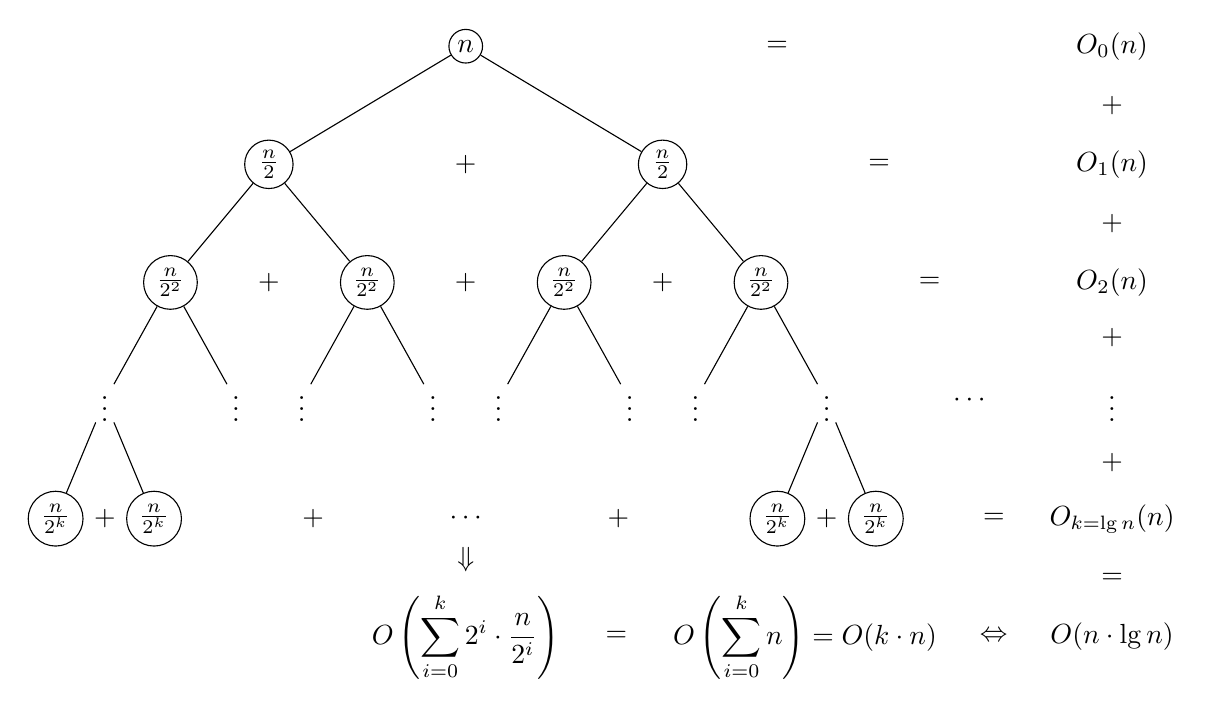
\begin{tikzpicture}[level/.style={sibling distance=50mm/#1}]
	\node [circle,draw] (z){$n$}
	child {node [circle,draw] (a) {$\frac{n}{2}$}
		child {node [circle,draw] (b) {$\frac{n}{2^2}$}
			child {node {$\vdots$}
				child {node [circle,draw] (d) {$\frac{n}{2^k}$}}
				child {node [circle,draw] (e) {$\frac{n}{2^k}$}}
			} 
			child {node {$\vdots$}}
		}
		child {node [circle,draw] (g) {$\frac{n}{2^2}$}
			child {node {$\vdots$}}
			child {node {$\vdots$}}
		}
	}
	child {node [circle,draw] (j) {$\frac{n}{2}$}
		child {node [circle,draw] (k) {$\frac{n}{2^2}$}
			child {node {$\vdots$}}
			child {node {$\vdots$}}
		}
		child {node [circle,draw] (l) {$\frac{n}{2^2}$}
			child {node {$\vdots$}}
			child {node (c){$\vdots$}
				child {node [circle,draw] (o) {$\frac{n}{2^k}$}}
				child {node [circle,draw] (p) {$\frac{n}{2^k}$}
					child [grow=right] {node (q) {$=$} edge from parent[draw=none]
						child [grow=right] {node (q) {$O_{k = \lg n}(n)$} edge from parent[draw=none]
							child [grow=up] {node (r) {$\vdots$} edge from parent[draw=none]
								child [grow=up] {node (s) {$O_2(n)$} edge from parent[draw=none]
									child [grow=up] {node (t) {$O_1(n)$} edge from parent[draw=none]
										child [grow=up] {node (u) {$O_0(n)$} edge from parent[draw=none]}
									}
								}
							}
							child [grow=down] {node (v) {$O(n \cdot \lg n)$}edge from parent[draw=none]}
						}
					}
				}
			}
		}
	};
	\path (a) -- (j) node [midway] {+};
	\path (b) -- (g) node [midway] {+};
	\path (k) -- (l) node [midway] {+};
	\path (k) -- (g) node [midway] {+};
	\path (d) -- (e) node [midway] {+};
	\path (o) -- (p) node [midway] {+};
	\path (o) -- (e) node (x) [midway] {$\cdots$}
	child [grow=down] {
		node (y) {$O\left(\displaystyle\sum_{i = 0}^k 2^i \cdot \frac{n}{2^i}\right)$}
		edge from parent[draw=none]
	};
	\path (q) -- (r) node [midway] {+};
	\path (s) -- (r) node [midway] {+};
	\path (s) -- (t) node [midway] {+};
	\path (s) -- (l) node [midway] {=};
	\path (t) -- (u) node [midway] {+};
	\path (z) -- (u) node [midway] {=};
	\path (j) -- (t) node [midway] {=};
	\path (y) -- (x) node [midway] {$\Downarrow$};
	\path (v) -- (y)
	node (w) [midway] {$O\left(\displaystyle\sum_{i = 0}^k n\right) = O(k \cdot n)$};
	\path (q) -- (v) node [midway] {=};
	\path (e) -- (x) node [midway] {+};
	\path (o) -- (x) node [midway] {+};
	\path (y) -- (w) node [midway] {$=$};
	\path (v) -- (w) node [midway] {$\Leftrightarrow$};
	\path (r) -- (c) node [midway] {$\cdots$};
\end{tikzpicture}}

%\subsection{title}
\section{Ví dụ 3 - vẽ lưới và tọa độ cực}	
\begin{center}

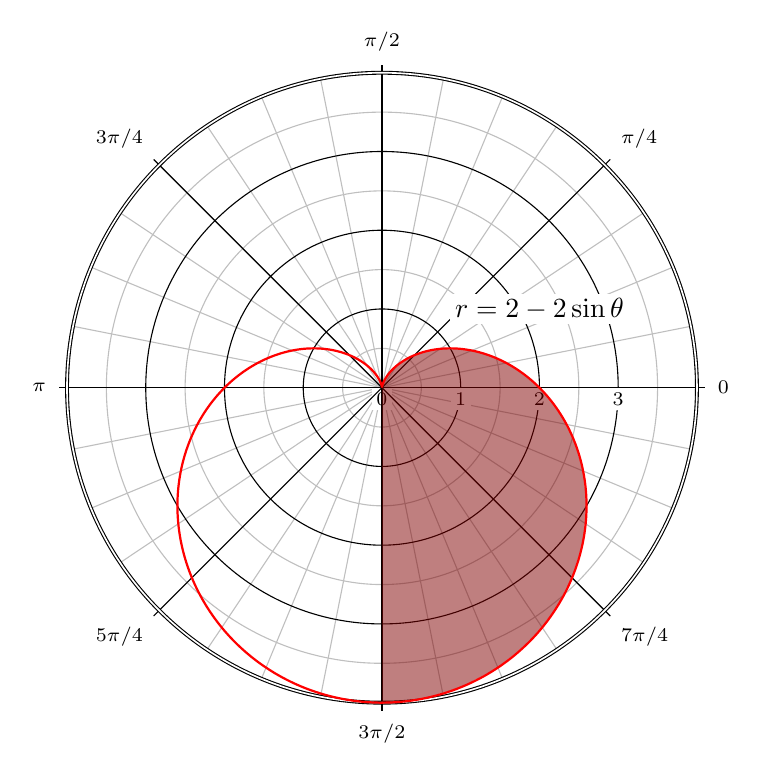
\begin{tikzpicture}[>=latex]
\foreach \ang in {0,...,31} {
	\draw [lightgray] (0,0) -- (\ang * 180 / 16:4);
}

% Concentric circles and radius labels
\foreach \s in {0, 1, 2, 3} {
	\draw [lightgray] (0,0) circle (\s + 0.5);
	\draw (0,0) circle (\s);
	\node [fill=white] at (\s, 0) [below] {\scriptsize $\s$};
}

% Add the labels at multiples of pi/4
\foreach \ang/\lab/\dir in {
	0/0/right,
	1/{\pi/4}/{above right},
	2/{\pi/2}/above,
	3/{3\pi/4}/{above left},
	4/{\pi}/left,
	5/{5\pi/4}/{below left},
	7/{7\pi/4}/{below right},
	6/{3\pi/2}/below} {
	\draw (0,0) -- (\ang * 180 / 4:4.1);
	\node [fill=white] at (\ang * 180 / 4:4.2) [\dir] {\scriptsize $\lab$};
}

% The double-lined circle around the whole diagram
\draw [style=double] (0,0) circle (4);

\fill [fill=red!50!black, opacity=0.5] plot [domain=-pi/2:pi/2]
(xy polar cs:angle=\x r, radius= {2-2*sin(\x r)});
\draw [thick, color=red, domain=0:2*pi, samples=200, smooth]
plot (xy polar cs:angle=\x r, radius={2-2*sin(\x r)});
\node [fill=white] at (2,1) {$r=2-2\sin\theta$};

\end{tikzpicture} 
\end{center}
%\includepdf[pages=-,pagecommand={}]{BienBanThuNghiem.pdf}

\usetikzlibrary{arrows,automata}
\usetikzlibrary{positioning}


\tikzset{
	state/.style={
		rectangle,
		rounded corners,
		draw=black, very thick,
		minimum height=2em,
		inner sep=2pt,
		text centered,
	},
}


\section{Ví dụ 4 - câu lệnh vẽ sơ đồ nguyên lý}
\usetikzlibrary{decorations.pathmorphing} % for snake lines
\usetikzlibrary{matrix} % for block alignment
\usetikzlibrary{arrows} % for arrow heads
\usetikzlibrary{calc} % for manimulation of coordinates

% TikZ styles for drawing
\tikzstyle{block} = [draw,rectangle,thick,minimum height=2em,minimum width=2em]
\tikzstyle{sum} = [draw,circle,inner sep=0mm,minimum size=2mm]
\tikzstyle{connector} = [->,thick]
\tikzstyle{line} = [thick]
\tikzstyle{branch} = [circle,inner sep=0pt,minimum size=1mm,fill=black,draw=black]
\tikzstyle{guide} = []
\tikzstyle{snakeline} = [connector, decorate, decoration={pre length=0.2cm,
	post length=0.2cm, snake, amplitude=.4mm,
	segment length=2mm},thick, magenta, ->]

\renewcommand{\vec}[1]{\ensuremath{\boldsymbol{#1}}} % bold vectors
\def \myneq {\skew{-2}\not =} % \neq alone skews the dash	
	
\begin{center}
	
\begin{tikzpicture}[scale=1, auto, >=stealth']
	\small
	% node placement with matrix library: 5x4 array
	\matrix[ampersand replacement=\&, row sep=0.2cm, column sep=0.4cm] {
		%
		\node[block] (F1) {$\vec{u}_i = F_i(\{\widetilde{\vec{x}}_j\}_{j=1}^N)$}; \&
		\node[branch] (u1) {}; \&
		\&
		\node[block] (f1) {$\begin{matrix}
			\dot{\vec{x}}_i =
			f_i(\vec{x}_i,
			\textcolor{red}{\{\widetilde{\vec{x}}_j\}_{j \myneq i}},
			\vec{u}_i,
			t)\\
			\vec{y}_i =
			g_i(\vec{x}_i,
			\textcolor{blue}{\{\widetilde{\vec{x}}_j\}_{j \myneq i}},
			t)
			\end{matrix}$}; \& \\
		
		\&
		\&
		\&
		\node[block] (L1) {$\vec{e}_i(\vec{y}_i - \widetilde{\vec{y}}_i)$};\&
		\node [sum] (e1) {}; \\
		
		\&
		\&
		\node[sum] (v1) {}; \&
		\node[block] (o1) {$\begin{matrix}
			\dot{\widetilde{\vec{x}}}_i =
			\widetilde{f}_i(\widetilde{\vec{x}}_i,
			\textcolor{red}{\{\widetilde{\vec{x}}_j\}_{j \myneq i}},
			\vec{v}_i, t)\\
			\widetilde{\vec{y}}_i =
			g_i(\widetilde{\vec{x}}_i,
			\textcolor{blue}{\{\widetilde{\vec{x}}_j\}_{j \myneq i}},
			t)
			\end{matrix}$};
		\&
		\\
		\node[guide] (i1) {}; \& \& \& \& \\
	};
	
	% now link the nodes
	\draw [line] (F1) -- (u1);
	\draw [connector] (u1) -- node {$u_i$} (f1);
	\draw [connector] (f1) -| node[near end] {$\vec{y}_i$} (e1);
	\draw [connector] (e1) -- (L1);
	\draw [connector] (L1) -| (v1);
	\draw [connector] (v1) -- node {$\vec{v}_i$} (o1);
	\draw [connector] (u1) |- (v1);
	\draw [connector] (o1) -| node[pos=0.96] {$-$} node [near end, swap]
	{$\widetilde{\vec{y}}_i$} (e1);
	\draw [connector] (o1.south) -- ++(0,-.5cm) -| node [near start]
	{$\widetilde{\vec{x}}_i$} ($(F1.south) + (0.4cm, 0em)$);
	
	% draw the snake lines with offset (using the calc library)
	\draw [snakeline] ($(i1) - (0.4cm, -1cm)$) -- node
	{$\{\widetilde{\vec{x}}_j\}_{j \myneq i}$} ($(F1.south) - (0.4cm, 0em)$);
	
	\draw [snakeline, swap] ($(v1.east) - (1.0cm, 0.4cm)$) -- node
	{$\{\widetilde{\vec{x}}_j\}_{j \myneq i}$} ($(o1.west) - (0cm, 0.4cm)$);
	
	\draw [snakeline, swap] ($(u1.east) + (0.1cm, -0.4cm)$) -- node
	{$\{\widetilde{\vec{x}}_j\}_{j \myneq i}$} ($(f1.west) - (0cm, 0.4cm)$);
	
\end{tikzpicture}	
\end{center}
	
\section{ví dụ 5 - câu lệnh vẽ máy Oscilloscope}
\def\scl{0.6}%scaling factor of the picture

\begin{center}
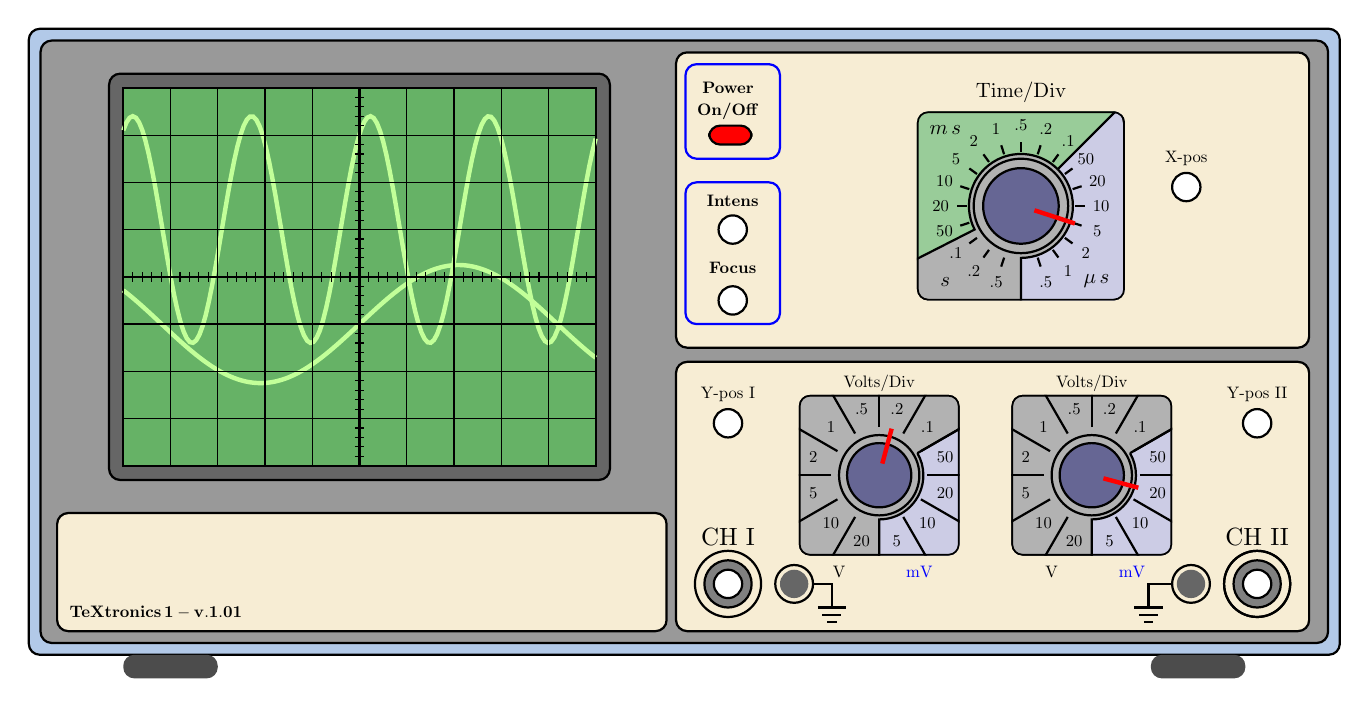
\begin{tikzpicture}[
scale=\scl,
controlpanels/.style={yellow!30!brown!20!,rounded corners,draw=black,thick},
screen/.style={green!50!black!60!,draw=black,thick},
trace/.style={green!60!yellow!40!, ultra thick},
smallbutton/.style={white,draw=black, thick},
axes/.style={thick}]
\fill[green!30!blue!30!,rounded corners,draw=black,thick](0,0)
rectangle (27.75,13.25);
\fill[fill=black!40!,draw=black,thick,rounded corners](0.25,0.25)
rectangle (27.5,13.00);
% Screen, centered around the origin then shifted for easy plotting
\begin{scope}[xshift=7cm,yshift=8cm,samples=150]
\fill[black!60!,rounded corners,draw=black,thick](-5.3,-4.3)
rectangle (5.3,4.3);
\fill[screen] (-5.0,-4.0) rectangle (5.0,4.0);
\draw[trace] plot(\x,{1+2.4*sin((2.5*\x +1) r)}); % r for radians...
\draw[trace] plot(\x,{-1+1.25*sin((0.75*\x) r});
\draw[thin] (-5.0,-4.0) grid (5.0,4.0);
\draw[axes] (-5,0)--(5,0); % Time axis
\draw[axes] (0,-4)--(0,4);
\foreach \i in {-4.8,-4.6,...,4.8} \draw (\i,-0.1)--(\i,0.1);
\foreach \i in {-3.8,-3.6,...,3.8} \draw (-0.1,\i)--(0.1,\i);
\end{scope}
% Feet
\fill[black!70!,rounded corners,xshift=2cm] (0,-.5) rectangle (2,0);
\fill[black!70!,rounded corners,xshift=23.75cm] (0,-.5) rectangle (2,0);
% Lower left panel
\fill[controlpanels] (0.6,0.5) rectangle (13.5,3.0);
\path (0.8,0.9) node[scale=\scl,right]{$\mathbf{TeXtronics\,1 - v.1.01}$};
% Lower right panel
\fill[controlpanels] (13.7,0.5) rectangle (27.1,6.2);
%Channels
% CH I
\draw[thick] (14.8,1.5) circle (0.7cm);
\fill[gray,draw=black,thick] (14.8,1.5) circle (0.5cm);
\fill[white,draw=black,thick] (14.8,1.5) circle (0.3cm);
\node[scale={1.5*\scl}] at (14.8,2.5) {CH I};
\draw[thick] (16.2,1.5) circle (0.4cm);
\fill[black!60!] (16.2,1.5) circle (0.3cm);
\draw[thick] (16.6,1.5) --(17,1.5)--(17,1.0);
\draw[thick] (16.7,1.0)--(17.3,1.0);
\draw[thick] (16.8,0.85)--(17.2,0.85);
\draw[thick] (16.9,0.70)--(17.1,0.70);
\draw[thick] (26.0,1.5) circle (0.7cm);
% CH II
\fill[gray,draw=black,thick] (26,1.5) circle (0.5cm);
\fill[white,draw=black,thick] (26,1.5) circle (0.3cm);
\node[scale={1.5*\scl}] at (26,2.5) {CH II};
\draw[thick] (24.6,1.5) circle (0.4cm);
\fill[black!60!] (24.6,1.5) circle (0.3cm);
\draw[thick] (24.2,1.5) --(23.7,1.5)--(23.7,1.0);
\draw[thick] (23.4,1.0)--(24.0,1.0);
\draw[thick] (23.5,0.85)--(23.9,0.85);
\draw[thick] (23.6,0.70)--(23.8,0.70);
\draw[thick] (26.0,1.5) circle (0.7cm);
% Y-pos
\fill[smallbutton] (14.8,4.9) circle (0.3cm);
\node[scale={\scl}] at (14.8,5.5) {Y-pos I};
\fill[smallbutton] (26.0,4.9) circle (0.3cm);
\node[scale={\scl}] at (26.0,5.5) {Y-pos II};
% Volt/div the foreach loop draws the two buttons
\foreach \i / \b in {18/75,22.5/345}{
	%Second parameter of the loop is the angle of the index mark 
	\begin{scope}[xshift=\i cm,yshift=3.8cm,scale=0.85]
	\node[scale=\scl] at (0,2.3) {Volts/Div};
	\node[scale=\scl,black] at (-1,-2.4) {V};
	\node[scale=\scl,blue]  at (1,-2.4) {mV};
	\clip[rounded corners] (-2,-2) rectangle (2,2);
	\fill[black!30!,rounded corners,draw=black,thick] (-2,-2)
	rectangle (2,2);
	\fill[blue!50!black!20!,draw=black,thick]
	(30:1.1)--(30:3)--(3,-3)--(-90:3)--(-90:1.1) arc (-90:30:1.1);
	\draw[very thick,rounded corners](-2,-2) rectangle (2,2);
	\draw[thick] (0,0) circle (1.0);
	\foreach \i in {0,30,...,330}
	\draw[thick] (\i:1.2)--(\i:2.5);
	\foreach \i/\j in {15/50,45/.1,75/.2,105/.5,135/1,165/2,195/5,225/10,
		255/20,285/5,315/10,345/20} \node[scale=\scl,black] at (\i:1.7) {\j};
	\fill[blue!30!black!60!,draw=black,thick] (0,0) circle (0.8cm);
	% Here you set the right Volts/Div button
	\draw[ultra thick,red] (\b:0.3)--(\b:1.2);
	\end{scope}}
% Upper right panel
\fill[controlpanels] (13.7,6.5) rectangle (27.1,12.75);
%On-Off button
\draw[rounded corners,thick,blue] (13.9,10.5) rectangle (15.9,12.5);
\fill[fill=red,draw=black,thick,rounded corners] (14.4,10.8) rectangle (15.3,11.2);
\node[scale=\scl] at (14.8,12) {\textbf{Power}};
\node[scale=\scl] at (14.8,11.5) {\textbf{On/Off}};
% Focus-Intensity buttons
\draw[rounded corners,thick,blue] (13.9,7.0) rectangle (15.9,10.0);
\fill[smallbutton] (14.9,7.5) circle (0.3cm);
\node[scale=\scl] at (14.9,8.2) {\textbf{Focus}};
\fill[smallbutton] (14.9,9) circle (0.3cm);
\node[scale=\scl] at (14.9,9.6) {\textbf{Intens}};
% X-pos
\fill[smallbutton] (24.5,9.9) circle (0.3cm);
\node[scale={\scl}] at (24.5,10.5) {X-pos};
% Time/Div
\begin{scope}[xshift=21cm,yshift=9.5cm,scale=1]
\node[scale={1.25*\scl}]  at (0,2.4) {Time/Div};
\clip[rounded corners] (-2.2,-2) rectangle (2.2,2);
\fill[black!30!,rounded corners,draw=black,thick] (-2.2,-2) rectangle (2.2,2);
\fill[blue!50!black!20!,draw=black,thick]
(45:1.1)--(45:3)--(3,-3)--(-90:3)--(-90:1.1) arc (-90:45:1.1);
\fill[green!50!black!40!,draw=black,thick]
(45:1.1)--(45:3) arc(45:207:3) --(207:1.1) arc (207:45:1.1);
\draw[very thick,rounded corners](-2.2,-2) rectangle (2.2,2);
\node[scale={1.25*\scl}] at (-1.6,-1.6) {$s$};
\node[scale={1.25*\scl}] at (1.6,-1.6) {$\mu{}\,s$};
\node[scale={1.25*\scl}] at (-1.6,1.6) {$m\,s$};
\draw[thick] (0,0) circle (1.0);
\foreach \i in {-72,-54,...,262} \draw[thick] (\i:1.15)--(\i:1.35);
\foreach \i/\j in {-72/.5,-54/1,-36/2,-18/5,0/10,18/20,36/50,54/.1,72/.2,90/.5,
	108/1,126/2,144/5,162/10,180/20,198/50,216/.1,234/.2,252/.5}
\node[scale=\scl,black] at (\i:1.7){\j};
\fill[blue!30!black!60!,draw=black,thick] (0,0) circle (0.8cm);
% Here you set the Time/Div button
\draw[ultra thick,red] (-18:0.3)--(-18:1.2);	
% X-pos
\end{scope}
\end{tikzpicture}
\end{center}

\section{ví dụ 6 - câu lệnh thể hiện tính chất của ánh sáng}
\usetikzlibrary{arrows}

	\begin{tikzpicture}[x={(0.866cm,-0.5cm)}, y={(0.866cm,0.5cm)}, z={(0cm,1cm)}, scale=1.0,
	%Option for nice arrows
	>=stealth, %
	inner sep=0pt, outer sep=2pt,%
	axis/.style={thick,->},
	wave/.style={thick,color=#1,smooth},
	polaroid/.style={fill=black!60!white, opacity=0.3},
	]
	% Colors
	\colorlet{darkgreen}{green!50!black}
	\colorlet{lightgreen}{green!80!black}
	\colorlet{darkred}{red!50!black}
	\colorlet{lightred}{red!80!black}
	
	% Frame
	\coordinate (O) at (0, 0, 0);
	\draw[axis] (O) -- +(14, 0,   0) node [right] {x};
	\draw[axis] (O) -- +(0,  2.5, 0) node [right] {y};
	\draw[axis] (O) -- +(0,  0,   2) node [above] {z};
	
	\draw[thick,dashed] (-2,0,0) -- (O);
	
	% monochromatic incident light with electric field
	\draw[wave=blue, opacity=0.7, variable=\x, samples at={-2,-1.75,...,0}]
	plot (\x, { cos(1.0*\x r)*sin(2.0*\x r)}, { sin(1.0*\x r)*sin(2.0*\x r)})
	plot (\x, {-cos(1.0*\x r)*sin(2.0*\x r)}, {-sin(1.0*\x r)*sin(2.0*\x r)});
	
	\foreach \x in{-2,-1.75,...,0}{
		\draw[color=blue, opacity=0.7,->]
		(\x,0,0) -- (\x, { cos(1.0*\x r)*sin(2.0*\x r)}, { sin(1.0*\x r)*sin(2.0*\x r)})
		(\x,0,0) -- (\x, {-cos(1.0*\x r)*sin(2.0*\x r)}, {-sin(1.0*\x r)*sin(2.0*\x r)});
	}
	
	\filldraw[polaroid] (0,-2,-1.5) -- (0,-2,1.5) -- (0,2,1.5) -- (0,2,-1.5) -- (0,-2,-1.5)
	node[below, sloped, near end]{Polaroid};%
	
	%Direction of polarization
	\draw[thick,<->] (0,-1.75,-1) -- (0,-0.75,-1);
	
	% Electric field vectors
	\draw[wave=blue, variable=\x,samples at={0,0.25,...,6}]
	plot (\x,{sin(2*\x r)},0)node[anchor=north]{$\vec{E}$};
	
	%Polarized light between polaroid and thin section
	\foreach \x in{0, 0.25,...,6}
	\draw[color=blue,->] (\x,0,0) -- (\x,{sin(2*\x r)},0);
	
	\draw (3,1,1) node [text width=2.5cm, text centered]{Ánh sáng phân cực};
	
	%Crystal thin section
	\begin{scope}[thick]
	\draw (6,-2,-1.5) -- (6,-2,1.5) node [above, sloped, midway]{Lớp tinh thể}
	-- (6, 2, 1.5) -- (6, 2, -1.5) -- cycle % First face
	(6,  -2, -1.5) -- (6.2, -2,-1.5)
	(6,   2, -1.5) -- (6.2,  2,-1.5)
	(6,  -2,  1.5) -- (6.2, -2, 1.5)
	(6,   2,  1.5) -- (6.2,  2, 1.5)
	(6.2,-2, -1.5) -- (6.2, -2, 1.5) -- (6.2, 2, 1.5) 
	-- (6.2, 2, -1.5) -- cycle; % Second face
	
	%Optical indices
	\draw[darkred, ->]       (6.1, 0, 0) -- (6.1, 0.26,  0.966) node [right] {$n_{g}'$}; % index 1
	\draw[darkred, dashed]   (6.1, 0, 0) -- (6.1,-0.26, -0.966); % index 1
	\draw[darkgreen, ->]     (6.1, 0, 0) -- (6.1, 0.644,-0.173) node [right] {$n_{p}'$}; % index 2
	\draw[darkgreen, dashed] (6.1, 0, 0) -- (6.1,-0.644, 0.173); % index 2
	\end{scope}
	
	%Rays leaving thin section
	\draw[wave=darkred,   variable=\x, samples at={6.2,6.45,...,12}] 
	plot (\x, {0.26*0.26*sin(2*(\x-0.5) r)},  {0.966*0.26*sin(2*(\x-0.5) r)});  %n'g-oriented ray
	\draw[wave=darkgreen, variable=\x, samples at={6.2,6.45,...,12}]
	plot (\x, {0.966*0.966*sin(2*(\x-0.1) r)},{-0.26*0.966*sin(2*(\x-0.1) r)}); %n'p-oriented ray
	\draw (10,1,1) node [text width=2.5cm, text centered] {Ánh sáng phân cực và lệch pha };
	
	\foreach \x in{6.2,6.45,...,12} {
		\draw[color=darkgreen, ->] (\x, 0, 0) --
		(\x, {0.966*0.966*sin(2*(\x-0.1) r)}, {-0.26*0.966*sin(2*(\x-0.1) r)});
		\draw[color=darkred,   ->] (\x, 0, 0) --
		(\x, {0.26*0.26*sin(2*(\x-0.5) r)}, {0.966*0.26*sin(2*(\x-0.5) r)});
	}
	
	%Second polarization
	\draw[polaroid]   (12, -2,  -1.5) -- (12, -2,   1.5)  %Polarizing filter
	node [above, sloped,midway] {Polaroid} -- (12, 2, 1.5) -- (12, 2, -1.5) -- cycle;
	\draw[thick, <->] (12, -1.5,-0.5) -- (12, -1.5, 0.5); %Polarization direction
	
	%Light leaving the second polaroid
	\draw[wave=lightgreen,variable=\x, samples at={12, 12.25,..., 14}]
	plot (\x,{0}, {0.966*0.966*0.26*sin(2*(\x-0.5) r)}); %n'g polarized ray
	\draw[wave=lightred,  variable=\x, samples at={12, 12.25,..., 14}]
	plot (\x,{0}, {-0.26*0.966*sin(2*(\x-0.1) r)});      %n'p polarized ray
	
	\node[align=justify, text width=14cm, anchor=north west, yshift=-2mm] at (current bounding box.south west)
	{};
	\end{tikzpicture}
	
\section{ví dụ 7 - câu lệnh vẽ Màng ion}	
\begin{center}

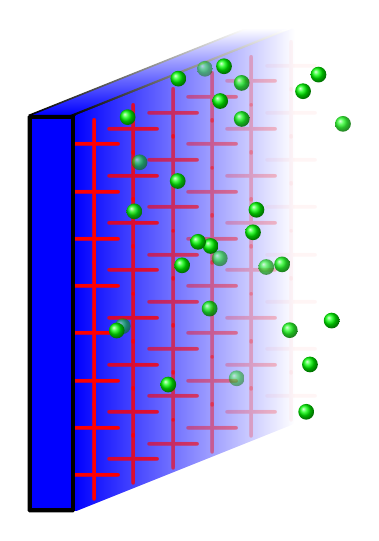
\begin{tikzpicture}[x=1cm, y=1cm]
\begin{scope}[every node/.append style={
	yslant=0,xslant=0},yslant=0,xslant=2.5
]
\shade[bottom color = black, top color = white] (-12.54, 5)
rectangle +(0.1, 1.1);
\shade[bottom color = blue, top color = white] (-12.48,5)
rectangle +(0.5,1.1);
\shade[bottom color = black, top color = white] (-12, 4.98)
rectangle +(0.1, 1.1);
\end{scope}

\begin{scope}[every node/.append style={
	yslant=0,xslant=0},yslant=0.4,xslant=0
]
\shade[left color = blue, right color = white, rounded corners=1]
(0.54,-0.26) rectangle +(2.8,5.03);
\foreach \x in {0.8,1.3,...,3.3}{
	\foreach \y in {0.1, 0.7,..., 4.8}{
		\pgfmathsetmacro{\val}{1-(\x-0.8)/2.6}
		\node [color = red, opacity =\val] at (\x ,\y) {\Huge{\textbf +}};
	}
}
\end{scope}

\pgfmathsetseed{10}

\foreach \i in {1,2,...,30}{
	%    \pgfmathsetmacro{\x}{(rand*0.5 + 1)*4 + 1}
	%    \pgfmathsetmacro{\y}{(rand*0.5 + 1)*3.9 + 2 }
	\pgfmathsetmacro{\x}{(rand*0.5 + 1)*3 - 0.5}
	\pgfmathsetmacro{\y}{(rand*0.5 + 1)*4.7-1.2}
	%    \pgfmathsetmacro{\opacVal}{0.95*(\x-2.5)/4 + rand*0.05}
	\pgfmathsetmacro{\opacVal}{rand*0.5+1}
	\shade [ball color = green, opacity = \opacVal] (\x,\y) circle (0.1);
}

\fill [fill = black,rounded corners= 0.6] (-0.05,-0.05)
rectangle +(0.6,5.05);
\fill [fill = blue] (0,0) rectangle +(0.5,4.95);
\end{tikzpicture}
	
\end{center}

\section{ví dụ 8 - câu lệnh vẽ tải trọng}

% Vector Styles
\tikzstyle{load}   = [ultra thick,-latex]
\tikzstyle{stress} = [-latex]
\tikzstyle{dim}    = [latex-latex]
\tikzstyle{axis}   = [-latex,black!55]

% Drawing Views
\tikzstyle{isometric}=[x={(0.710cm,-0.410cm)},y={(0cm,0.820cm)},z={(-0.710cm,-0.410cm)}]
\tikzstyle{dimetric} =[x={(0.935cm,-0.118cm)},y={(0cm,0.943cm)},z={(-0.354cm,-0.312cm)}]
\tikzstyle{dimetric2}=[x={(0.935cm,-0.118cm)},z={(0cm,0.943cm)},y={(+0.354cm,+0.312cm)}]
\tikzstyle{trimetric}=[x={(0.926cm,-0.207cm)},y={(0cm,0.837cm)},z={(-0.378cm,-0.507cm)}]

	\begin{center}
		\begin{tikzpicture}
		\node (origin) at (0,0) {}; % shift relative baseline
		\coordinate (O) at (2,3);
		\draw[fill=gray!10] (O) circle (1);
		\draw[fill=white] (O) circle (0.75) node[below,yshift=-1.125cm] {Mặt cắt};
		\draw[dim] (O) ++(-0.75,0) -- ++(1.5,0) node[midway,above] {$d_i$};
		\draw[dim] (O) ++(-1,1.25) -- ++(2,0) node[midway,above] {$d_o$}; 
		\foreach \x in {-1,1} {
			\draw (O) ++(\x,0.25) -- ++(0,1.25);
		}
		\end{tikzpicture}%
		\begin{tikzpicture}[dimetric2]
		\coordinate (O) at (0,0,0);
		\draw[axis] (O) -- ++(6,0,0) node[right] {$x$};
		\draw[axis] (O) -- ++(0,6,0) node[above right] {$y$};
		\draw[axis] (O) -- ++(0,0,6) node[above] {$z$};
		\draw[fill=gray!50] (0,0,-0.5) circle (0.5); 
		\fill[fill=gray!50] (-0.46,-0.2,-0.5) -- (0.46,0.2,-0.5) -- (0.46,0.2,0) -- (-0.46,-0.2,0) -- cycle;
		\draw[fill=gray!20] (O) circle (0.5);
		\draw (0.46,0.2,-0.5) -- ++(0,0,0.5) node[below right,pos=0.0] {Giá đỡ cố định};
		\draw (-0.46,-0.2,-0.5) -- ++(0,0,0.5);
		\draw[fill=gray!10] (O) circle (0.2);
		\fill[fill=gray!10] (-0.175,-0.1,0) -- (0.175,0.1,0) -- ++(0,0,4) -- (-0.175,-0.1,4) -- cycle;
		\draw (-0.175,-0.1,0) -- ++(0,0,4);
		\draw (0.175,0.1,0) -- ++(0,0,4) node[right,midway] {Thép};
		\draw (4,0,3.95) -- ++(0,0,-1);
		\foreach \z in {0.5,0.75,...,5} {
			\draw[-latex] (-2*\z/5-0.2,0,\z) -- (-0.2,0,\z);
		}
		\draw[load] (0,0,4) -- ++(0,0,-1.25) node[right,xshift=0.1cm] {$F_{z1}$};
		\draw[fill=gray!20] (-0.25,-0.25,5) -- (4,-0.25,5) -- (4,+0.25,5) -- (-0.25,+0.25,5) -- cycle; 
		\draw[fill=gray!50] (+4.00,-0.25,4) -- (4,+0.25,4) -- (4,+0.25,5) -- (+4.00,-0.25,5) -- cycle; 
		\draw[fill=gray!10] (-0.25,-0.25,4) -- (4,-0.25,4) -- (4,-0.25,5) -- (-0.25,-0.25,5) -- cycle; 
		\draw (4.05,0,4) -- ++(1,0,0);
		\draw (4.05,0,5) -- ++(1,0,0);
		\draw[dim] (4.5,0,0) -- ++(0,0,4) node[midway,right] {$h_1$};
		\draw[dim] (4.5,0,4) -- ++(0,0,1) node[midway,right] {$h_2$};
		\draw[dim] (0,0,3.4) -- ++(4,0,0) node[midway,below] {$b_2$};
		\coordinate (P) at (2,-0.25,4.5);
		\draw (P) -- ++(0,0,0.25);
		\draw (P) -- ++(0.25,0,0);
		\draw[dim] (2.125,-0.25,4.5) -- ++(0,0,-0.5) node[midway,right] {$z_1$};
		\draw[dim] (2,-0.25,4.625) -- ++(-2,0,0) node[midway,below] {$x_1$};
		\draw[load] (2,-2.45,4.5) -- ++(0,2.2,0) node[pos=0.0,right,xshift=0.08cm] {$F_{y1}$};
		\draw[axis,dashed,-] (O) -- (0,0,5);
		\draw (0,0,5.5) -- ++(4,0,0) node[midway,above] {$w_{z}$};
		\foreach \x in {0,0.25,...,4} {
			\draw[-latex] (\x,0,5.5) -- ++(0,0,-0.5);
		}
		\draw (-0.2,0,0) -- ++(-2,0,5) node[above,xshift=0.5cm] {$w_{x}=\frac{z}{h_1+h_2} w_0$};
		\end{tikzpicture} %
	\end{center}

\section{Ví dụ 9 - vẽ biểu đồ thời gian}

\newcounter{wavenum}

\setlength{\unitlength}{1cm}
% advance clock one cycle, not to be called directly
\newcommand*{\clki}{
	\draw (t_cur) -- ++(0,.3) -- ++(.5,0) -- ++(0,-.6) -- ++(.5,0) -- ++(0,.3)
	node[time] (t_cur) {};
}

\newcommand*{\bitvector}[3]{
	\draw[fill=#3] (t_cur) -- ++( .1, .3) -- ++(#2-.2,0) -- ++(.1, -.3)
	-- ++(-.1,-.3) -- ++(.2-#2,0) -- cycle;
	\path (t_cur) -- node[anchor=mid] {#1} ++(#2,0) node[time] (t_cur) {};
}

% \known{val}{length}
\newcommand*{\known}[2]{
	\bitvector{#1}{#2}{white}
}

% \unknown{length}
\newcommand*{\unknown}[2][XXX]{
	\bitvector{#1}{#2}{black!20}
}

% \bit{1 or 0}{length}
\newcommand*{\bit}[2]{
	\draw (t_cur) -- ++(0,.6*#1-.3) -- ++(#2,0) -- ++(0,.3-.6*#1)
	node[time] (t_cur) {};
}

% \unknownbit{length}
\newcommand*{\unknownbit}[1]{
	\draw[ultra thick,black!50] (t_cur) -- ++(#1,0) node[time] (t_cur) {};
}

% \nextwave{name}
\newcommand{\nextwave}[1]{
	\path (0,\value{wavenum}) node[left] {#1} node[time] (t_cur) {};
	\addtocounter{wavenum}{-1}
}

% \clk{name}{period}
\newcommand{\clk}[2]{
	\nextwave{#1}
	\FPeval{\res}{(\wavewidth+1)/#2}
	\FPeval{\reshalf}{#2/2}
	\foreach \t in {1,2,...,\res}{
		\bit{\reshalf}{1}
		\bit{\reshalf}{0}
	}
}

% \begin{wave}[clkname]{num_waves}{clock_cycles}
\newenvironment{wave}[3][clk]{
	\begin{tikzpicture}[draw=black, yscale=.7,xscale=1]
	\tikzstyle{time}=[coordinate]
	\setlength{\unitlength}{1cm}
	\def\wavewidth{#3}
	\setcounter{wavenum}{0}
	\nextwave{#1}
	\foreach \t in {0,1,...,\wavewidth}{
		\draw[dotted] (t_cur) +(0,.5) node[above] {t=\t} -- ++(0,.4-#2);
		\clki
	}
}{\end{tikzpicture}}

%%% End of timing.sty

	\begin{wave}{13}{5}
		\nextwave{req\_addr} \bit{0}{.2} \bit{1}{1} \bit{0}{3} \bit{1}{1} \bit{0}{.8}
		\nextwave{inst\_addr} \unknown[X]{.5} \known{addr}{1} \unknown{4.5}
		\nextwave{link\_addrs} \unknown{1.2} \known{map}{1} \unknown{3.8}
		\nextwave{link\_load} \unknown{2.2} \known{vam}{1} \unknown{2.8}
		\nextwave{link\_load\_r} \unknown{3.1} \known{val}{1} \unknown{1.9}
		\nextwave{simulate} \bit{0}{3.1} \bit{1}{1} \bit{0}{1.9}
		\nextwave{output} \unknown{3.3} \known{}{.5} \known{}{.5} \unknown{1.7}
		\nextwave{prev\_output} \unknown{3.2} \known{old}{1} \unknown{1.8}
		\nextwave{differs} \unknownbit{3.3} \bit{1}{.5} \bit{1}{.4} \unknownbit{1.8}
		\nextwave{differs\_r} \unknownbit{4.1} \bit{1}{1} \unknownbit{.9}
		\nextwave{dep\_addr} \unknown{4.2} \known{dep}{1} \unknown[X]{.8}
		\nextwave{req} \unknown{4.3} \known{req}{1} \unknown[X]{.7}
	\end{wave}
